\documentclass[tightenline,notitlepage,nofootinbib]{revtex4-1}

\bibliographystyle{plainnat}
%\DeclareOption{nofootinbib}{\@booleanfalse\footinbib@sw}

%\@booleanfalse\footinbib@sw

\usepackage{graphicx}
\usepackage{amsmath}
\usepackage{subcaption}
\usepackage{sidecap}
\usepackage{empheq}
\usepackage{cleveref}


\DeclareMathOperator{\erf}{Erf}
\DeclareMathOperator{\trace}{Tr}

\newcommand{\spinup}{\uparrow}
\newcommand{\spindown}{\downarrow}
\newcommand{\KSAE}{{I}}
\newcommand{\qav}[1]{\langle {#1} \rangle}
\newcommand*{\ket}[1]{\left \lvert {#1} \right \rangle}
\newcommand*{\bra}[1]{\left \langle {#1} \right \rvert}
\newcommand{\comm}[1]{{ \textbf{#1} }}



\begin{document}
  \title{An upgrade study of chargino detection with finer mass splittings.}
  \author{Janis Erdmanis \\ graphitewriter@gmail.com}
%  \email{akels14@gmail.com}
  \date{August 2016}
  \maketitle

  \section{Introduction}

  In the Standard Model (SM) Higgs mass is highly sensitive to the details of the physics at high-energy \cite{Barbieri}. Unless we accept big number cancellations, SM does not work well with naturalness principle which leads us to beyond SM (BSM) physics. This issue is resolved in supersimmetry (SUSY) introducing new particles, new processes at higher energies \cite{Carlos}. With a present data from large hardron collider (LHC) \cite{PhysRevD.93.052002} we know that all SUSY particles should be heavy except higgsino, where lower bound is established from LEP\footnote{Large electron positron accelerator.} $100~\rm{GeV}$. On the other hand for naturalness principle to hold higgsino mass has upper bound of about $1 ~\rm{TeV}$. Here we consider possibility to push lower bound of higgsino mass with high luminosity LHC data from ATLAS experiment \cite{HLLHC,ATLASCOL-2008}, therefore we initially consider higgsino mass to be $m_{h}=100~\rm{GeV}$ and its mass splittings $\Delta m_h = 5~\rm{GeV}$ (see \cref{fig:basic}).

Similarly as in previous studies \cite{PhysRevD.89.075007} here we are considering chargino, neutralino $\tilde \chi_1^{+},~\tilde \chi_1^{-}$ production which decays to neutralinos, neutrinos and soft leptons (see \cref{fig:basic}). These leptons are buried in SM background coming mainly from $pp\to \tau \tau + j$, $pp\to t \bar t + j$, $pp \to WW + j$ as thy have comparable cross-section as a signal (see \cref{tab:cross}). Also in our analysis we include process $pp \to W +j$ which although produces one soft lepton it has a large cross-section and therefore considerable chance for incorrectly detecting second lepton coming from jet (fake leptons). 
\begin{figure}[!ht]
    \centering
    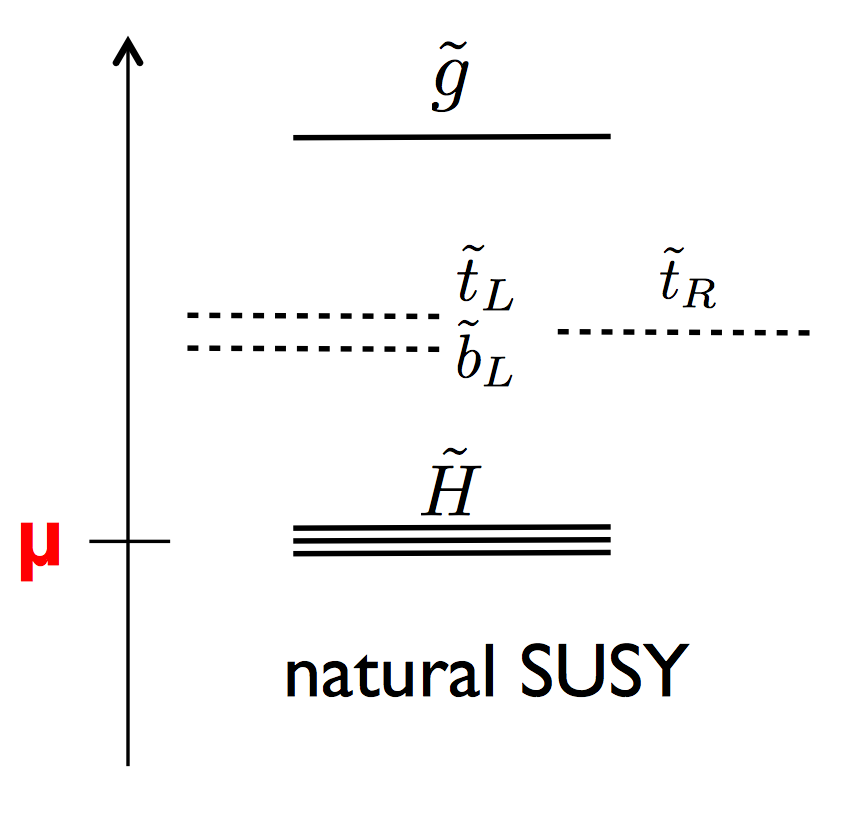
\includegraphics[width=0.25\textwidth]{splittings.png}
    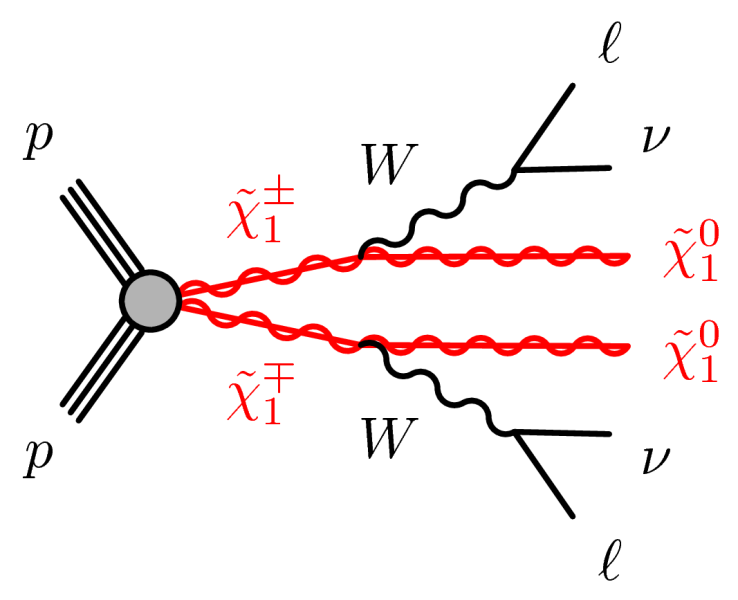
\includegraphics[width=0.25\textwidth]{C1C1.png}
    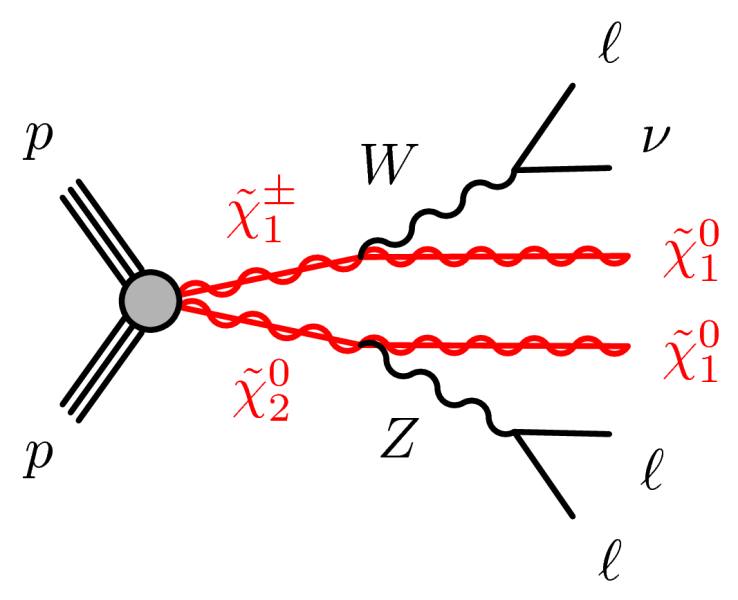
\includegraphics[width=0.25\textwidth]{C1N2.png}
    \caption{The SUSY particle mass spectrum with higgsino mass $\mu$ (left), 2 soft lepton SUSY signal (middle) and 3 soft lepton SUSY signal (right).}
    \label{fig:basic}
  \end{figure}

\begin{table}[!ht]
  \centering
  \begin{tabular}{ll}
    Process & $\sigma_{eff}$ \\
    \hline
    $pp\rightarrow \tau \tau + j$ & $47.6~\rm{pb}$\\
    $pp\rightarrow t \bar t + j$ & $ 8.9~\rm{pb}$\\
    $pp \rightarrow W + j$ &  $162~\rm{pb}$ \\
    $pp \rightarrow WW +j$ & $1.34~\rm{pb}$\\
    $pp \rightarrow \tilde \chi_1^{+}\tilde \chi_1^{-} + j \rightarrow WW + j$ & $2.8~\rm{pb}$\\
    $pp \rightarrow \tilde \chi_1^{+}\tilde \chi_2^{0} + j \rightarrow WZ + j$ & $5~\rm{pb}$\\
  \end{tabular}
  \caption{Cross sections at 14 TeV for the signal and background processes considered.}
  \label{tab:cross}
\end{table}
% MadGraph event generator for all theese processes is used from which we try to extract signal with appropriate selection.

To study and compare the signal and backgrounds, we turn to Monte Carlo. We simulate the hard processes for the signal and the major backgrounds with Madgraph 6. The parton-level events are then showered and hadronized with Pythia 8. 

\section{Simplified detector simulation}

Each simulated event consists of number of objects - particles, particle showers coming from quark hardronization (jets) and missing energy $E^{\rm{miss}}_T$ which we know from transverse momenta conservation. For each of these objects simulation gives us Lorentz four-vector and so we can calculate - energy, mass, momenta, transverse angle $\phi$\footnote{Because of symmetry, we are only concerned with angle differences between objects.}, pseidorapidity $\eta$.\footnote{Commonly used spatial coordinate describing angle of particle relative to beam axis. It is related to angle between momentum and beam axis with formula $\theta=2 \arctan (e^{-\eta})$.} as well as object labels - electron, positron, muon, lepton, jet, $b$-jet, photon. Unfortunately event reconstruction is limited by a detector imperfections, geometry, resolution and other properties. Because a real detector simulation is costly here we are going to use simplified model.

Firstly we smear object energies, masses, momenta, $\eta$, $\phi$, jet labels\footnote{Because of efficiency with which we can distinguish jets from $b$-jets.} of all objects (particles and jets) with corresponding performance functions for $200$ average interactions per bunch crossing as expected in HL LHC. Then from these smeared event particles we are able to detect only ones which hit detector $|\eta|<2.8$ and are energetic enough to trigger detector - for leptons  $p_{\rm{T}} > 5~\rm{GeV} $ and for jets $p_{\rm T}>50~\rm{GeV}$.

Because we are not interested in particles which comes from quark hardronization (jets) then we have to exclude particles which comes from jets. At overlap removal stage if lepton and jet are separated with less than $\Delta R = \sqrt{\Delta \phi^2 + \Delta \eta^2}<0.2$ and if transverse momenta of lepton is at least $50~ \%$ of transverse momenta of jet then we discard jet. For remaining objects if distance between jet and lepton is $\Delta R < 0.4$ we discard lepton assuming it belongs to the jet. We also assume that lepton belongs to jet if it has small energy and momenta compared to all particles around the cone. And eventually because we are not considering resonance processes at low energies we are removing low mass lepton pairs which have energy less than $12 ~\rm{GeV}$.

For checking this simplified detector simulation we plot transverse momentum of leading jet and leading lepton at different stages of algorithm (see figure \cref{fig:check}). For jets we see that smearing of variables indeed makes distribution broader (red line) where cut at $30~\rm{GeV}$ corresponds to undefined behavior of smearing function. Then some jets are removed at overlap removal stage while majority are discarded with $p_{\rm T}$ threshold (green line). Similarly for leading lepton we see considerable smearing (red line) and discarded leptons with $p_{\rm T}$ threshold and a little amount discarded at overlap removal stage (green line). 
\begin{figure}[!ht]
  \centering
  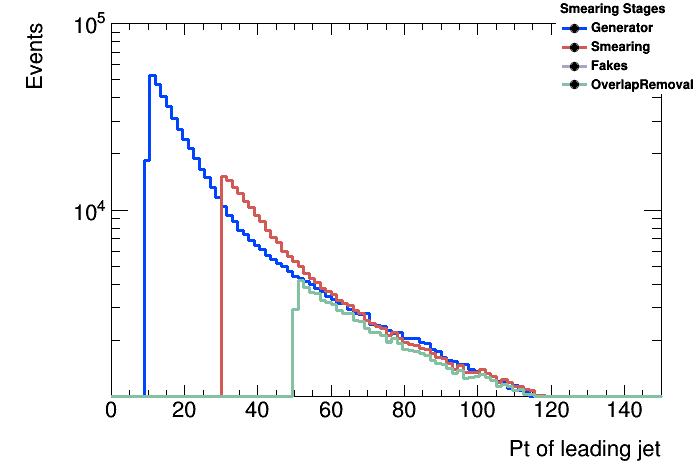
\includegraphics[width=0.45\textwidth]{h_PtJets1stStages.png}
  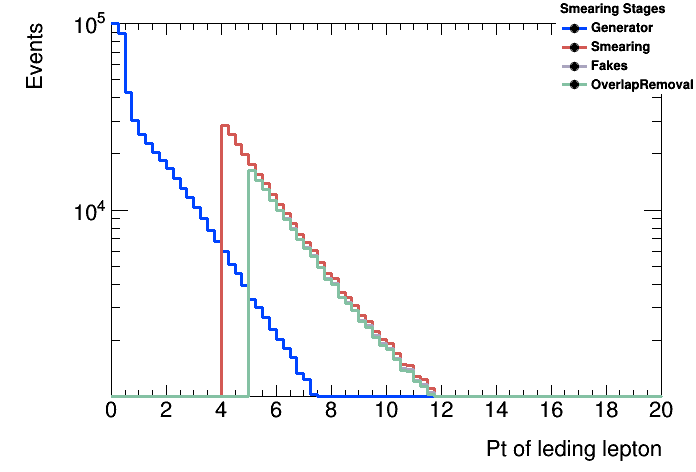
\includegraphics[width=0.45\textwidth]{h_PtEleMuo1stStages.png}
  \caption{Tests of smearing functions for signal sample C1C1 at different stages for leading jet $p_{\rm T}$ (left) and leading lepton $p_{\rm T}$ (right). Generator (blue line), smearing stage (red line) and overlap removal (green line).}
  \label{fig:check}
\end{figure}

% \begin{figure}[!ht]
%   \centering
%   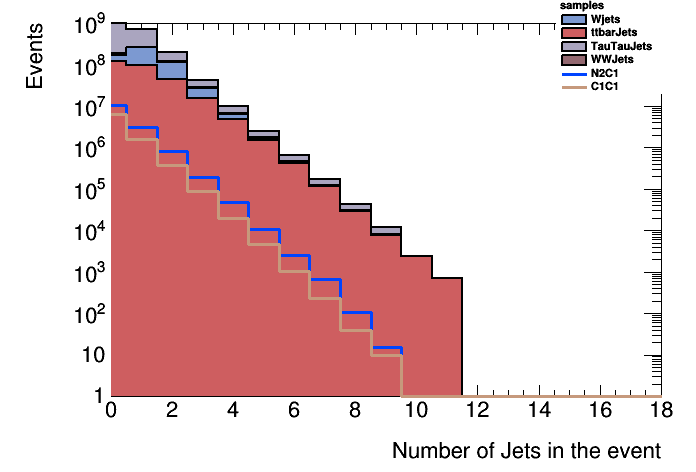
\includegraphics[width=0.25\textwidth]{h_NJet.png}
%   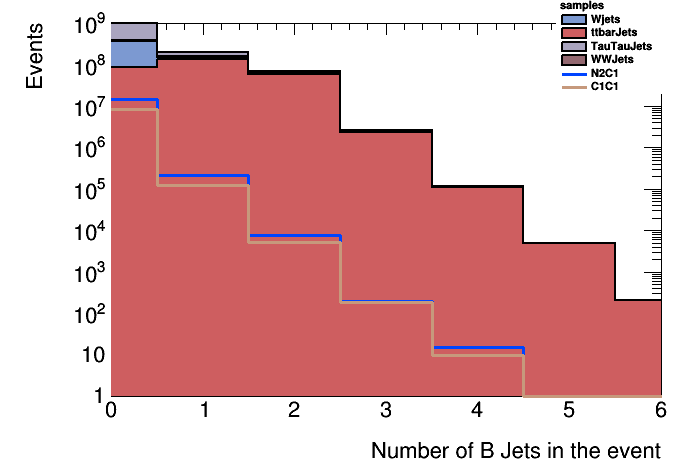
\includegraphics[width=0.25\textwidth]{h_NBJet.png}
%   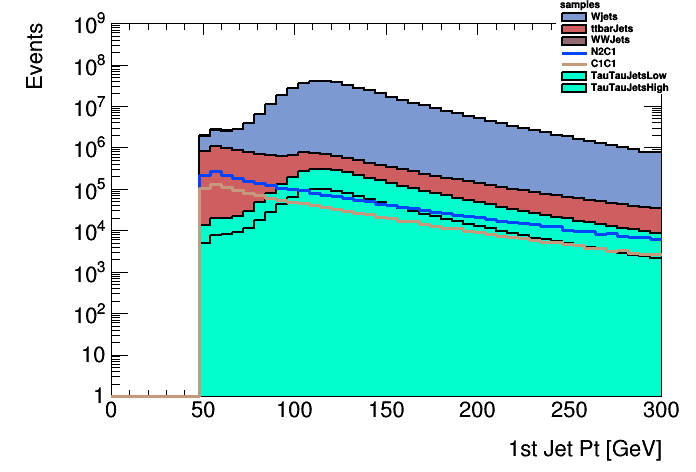
\includegraphics[width=0.25\textwidth]{h_PtJets1st.png}
%   \caption{Number of Jets, Bjets and leading jet transverse momentum.}
% \end{figure}

\section{Event selection}

%%% Writting more why I apply each requirement

Without any selection we have low signal and background relative ratio as in \cref{fig:nocuts} which also helps us to check the simulation. For example we see resonance for transverse mass at $90~\rm{GeV}$ for $pp \to W +j$ as expected. To increase signal ratio over background we are going to apply selection.
\clearpage
\begin{figure}[!ht]
  \centering
  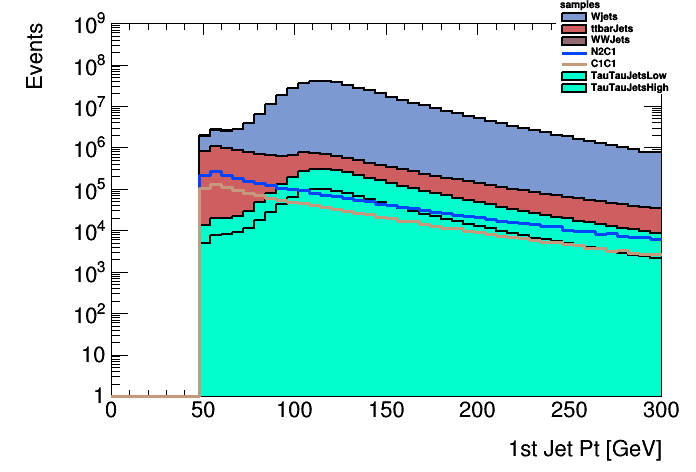
\includegraphics[width=0.3\textwidth]{h_PtJets1st.png}
  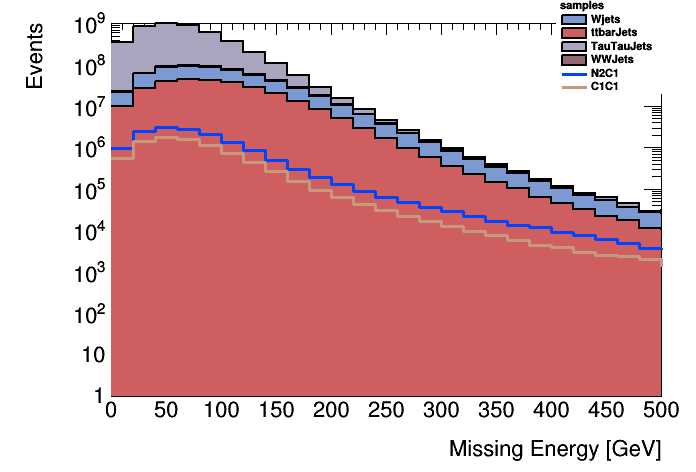
\includegraphics[width=0.3\textwidth]{h_MET.png}
  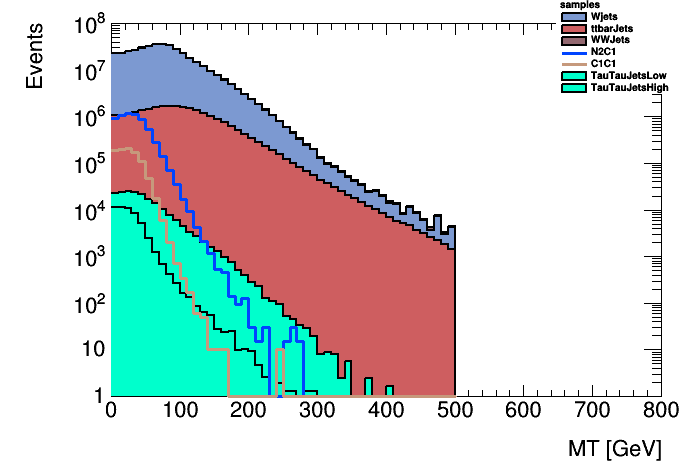
\includegraphics[width=0.3\textwidth]{h_MT.png}
  \caption{Missing energy (left), two leading lepton mass $m_{ll}$ (middle) and transverse mass (right). SUSY signals (blue and orange lines), background processes (filled green, red, blue). }
  \label{fig:nocuts}
\end{figure}

The signal (see \cref{fig:basic}) produces soft leptons (small transverse momenta) as well as some jets and neutrinos, neutralinos. The latter ones does not leave trace in ATLAS detector and so violates detected transverse momenta conservation which we measure with missing energy.  

When both neutralinos are forced to recoil against another object in the event - a jet in this case here - they lead to a large $E_T^{\rm{miss}}$ signature. In order to have such forced events we require single energetic jet which points backwards from missing energy as well we need large missing energy. Therefore the first requirements we impose
\begin{itemize}
\item Single jet with $p_{\rm T}>100~\rm{GeV}$;
\item $E_T^{\rm{miss}}>200~\rm{GeV}$;
\item $\Delta \Phi(E_T^{\rm{miss}},1st ~jet)>0.4$;
\end{itemize}

The requirement of single energetic jet also kills majority of $pp \to t \bar t + j$ background which is characterized by at least two hard jets. If we even more assume that event is $b$-tagged we can minimize this background without affecting the signal. Here we assume a $b$-tag efficiency of $80 \%$ which we apply at smearing stage.

Majority of background $pp \to W + j$ and $pp \to \tau \tau +j$ are killed if we apply veto for at least two leptons in the process\footnote{Although it would not be so easy for $pp \to W +j$ in real life since in this study we lack to add lepton fakes for each event.}. On the other hand background $pp \to WW + j$ did not survive previous selection therefore for minimizing background overall we apply selections
\begin{itemize}
\item No $b$-tagged jets;
\item At least 2 leptons\footnote{Because of simplified detector algorithm lepton energies are larger than $5~\rm{GeV}$ (look in ApplyPtEtaThresholds).}.
\end{itemize}
\begin{figure}[!ht]
  \centering
  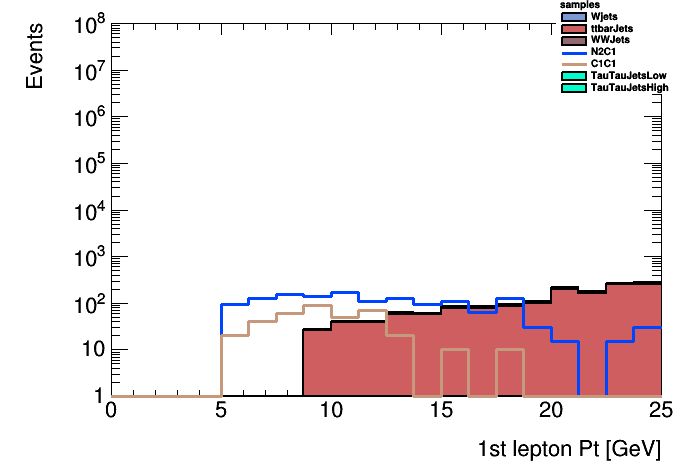
\includegraphics[width=0.3\textwidth]{h_PtMuons1st_2lead.png}
  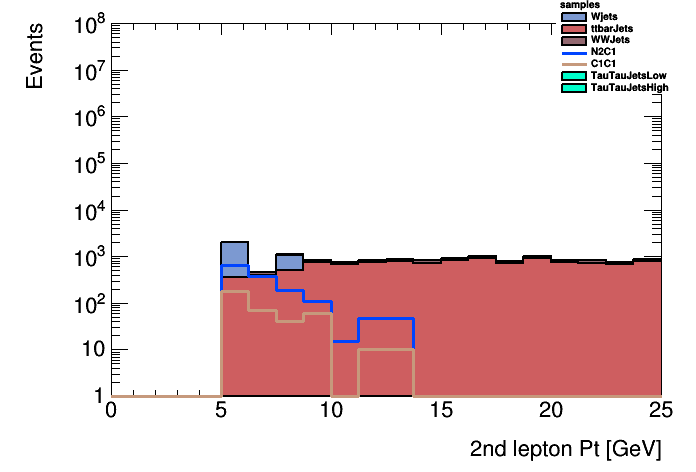
\includegraphics[width=0.3\textwidth]{h_PtMuons2nd_2lead.png}
  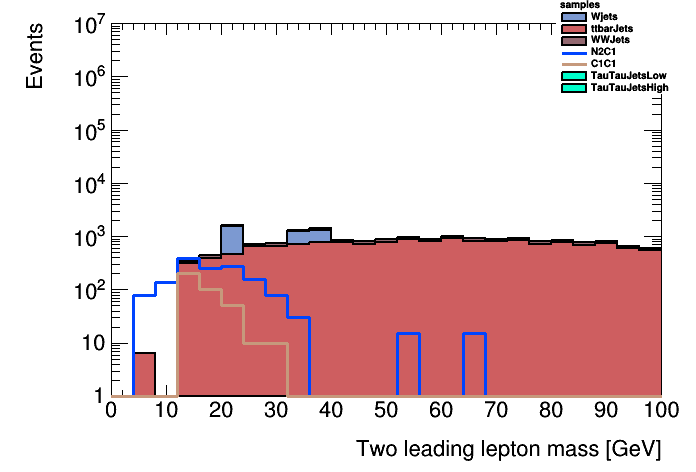
\includegraphics[width=0.3\textwidth]{h_llmass_2lead.png}
  \caption{The signal after selection. Leading lepton $p_{\rm T}$ (left), second leading lepton $p_{\rm T}$ (middle), first two leading lepton mass. SUSY signals (blue and orange lines), background processes (filled green, red, blue).}
  \label{fig:select}
\end{figure}

The results of this selection can be seen in in \cref{fig:select}. The signal over background ratio indeed has improved and has enough events at $L=3000 \rm{fb}^{-1}$ showing efficiency of present selection. Selecting events for leading lepton transverse momenta in range $5<p_{\rm T}<20~\rm{GeV}$ we calculate exact significance at \cref{tab:select}.
\begin{table}[!ht]
  \setlength{\tabcolsep}{12pt}
  \centering
  % \begin{tabular}{l|rrrrrr}
  %   & $\tau \tau$ & $t \bar t$ & $WW$ & $W$ & $\chi_1^{\pm} \chi_1^{\pm}$ &  $\chi_1^{\pm} \chi_2^0$ \\
  %   \hline
  %   $Events_{L=3000~\rm{fb}^{-1}}$  & 0 & $758 \pm 27$ & $67 \pm 8$ & 0 & $370 \pm 19$ & $1422 \pm 38$ \\
  %   $\sigma_{L=300~\rm{fb}^{-1}}$ & - & - & - & - & 0 & 0 \\
  %   $\sigma_{L=3000~\rm{fb}^{-1}}$ & - & - & - & - & 0 & 0 
                                                           %     \end{tabular}
  \begin{tabular}{l|rrr}
    Process & $\rm{Events}_{L=3000~\rm{fb}^{-1}}$ &$\sigma_{L=300~\rm{fb}^{-1}}$ & $\sigma_{L=3000~\rm{fb}^{-1}}$ \\
    \hline
    $\tau \tau$ & 0 & - & - \\
    $t \bar t$ & $758 \pm 27$ & - & - \\
    $WW$ & $67\pm8$ & - & - \\
    $W$ & 0 & - & - \\
    \hline
    TOTAL & $825 \pm 35$ & - & - \\
    \hline
    $\chi_1^{\pm} \chi_1^{\pm}$ & $370 \pm 19$ & 0 & 0 \\
    $\chi_1^{\pm} \chi_2^0$ & $1422 \pm 38$ & 0 & 0 
  \end{tabular}
  \caption{Significance calculation for leading lepton $p_{\rm T}$ in region $5<p_{\rm T}<20~\rm{GeV}$ luminosity $L=300~\rm{fb}^{-1}$ and $L=3000~\rm{fb}^{-1}$ with background uncertainty $30~\%$.
    %Number of events at $L=3000fb^-1$ after selection for leading lepton transverse momenta in region  for $L=3000fb$ and corresponding significance for luminosity $L=300 fb^-1$ and $L=3000 fb^-1$ with background uncertainty $30 \%$.
  }
  \label{tab:select}
\end{table}

\section{Conclusions}

%%% Extend conclusions
%%% Mentioning what are the results of this study, and perspectives (have a look at the other upgrade study).

In this study we have shown usefulness of HL LHC data for pushing bounds of higgsino masses previously set by LEP targeting soft leptons possibly coming from chargino and neutralino production by applying reasonable event selections. We have shown that single energetic jet which points backwards from large missing energy is indeed efficient selection and could be used as basis for more detailed studies. After adding veto for no $b$-jets and requiring at least 2 leptons we found that most significant contribution for background comes from $pp \to t \bar{t} + j$ where better understanding on how it can be minimized is needed.

With this selection we found that signal emerges most boldly for leading lepton transverse momenta which we used for significance calculation. With $L=3000~\rm{fb}^{-1}$ and background uncertainty $30 \%$ we found significance to be $...$ for $\chi_1^{\pm} \chi_1^{\pm}$ and $...$ for $\chi_1^{\pm} \chi_2^0$ which can (can't) be used as a tool for pushing lower bound of higgsino mass. However validness of this result can be greatly altered since our simplified detector simulation does not consider lepton fakes comming from large $pp \to W +j$ background. 

% \begin{itemize}
% \item With selection used in this report we are able to better distinguish signal from background processes.  
% \item SM process $pp \to t \bar t + j$ is not excluded efficiently enough with a present selection. A further study of how it can be minimized is needed. 
% \item The significance discovering higgsino particle with mass $100~\rm{GeV}$ at HL LHC is ... which is (not) enough for making discovery. 
% \end{itemize}

% \nocite{*}
%\bibliographystyle{unsrt}
\bibliography{bibliography}{9}
%\bibliographystyle{plain}
  \end{document}

%%% Local Variables:
%%% mode: latex
%%% TeX-master: t
%%% End:














